\documentclass[stu,12pt,floatsintext]{apa7}
\usepackage[american]{babel}
\usepackage{csquotes}
\usepackage{amsmath,amssymb}
\usepackage{graphicx}
\usepackage{booktabs}
\usepackage{float}
\usepackage{apacite}
\graphicspath{{figures/}}

\title{Geopolitical Risk Scoring and Anomaly Detection}
\shorttitle{Geopolitical Risk Scoring}
\author{Oussama Ennaciri}
\affiliation{Anderson College of Business and Computing, Regis University}
\course{MSDS692: Data Science Practicum}
\professor{Dr. Ghulam Mujtaba}
\duedate{27 June 2026}

\abstract{This project builds one system to measure and track geopolitical risk for each country. It has two parts. The first is a risk scorer. It learns the Geopolitical Risk index from a country's structural features, then gives a score to every country, including the ones with no published index. The second is an early warning detector. It watches monthly news signals and flags a country that is moving away from its own normal. I joined nine open sources into one country year table of 2,470 country years across 247 countries from 2015 to 2024. Of these, 440 across 44 countries have an official index. The scorer is an XGBoost model. It ranks countries it never saw at a Spearman correlation of 0.81, and it forecasts the next year at 0.91 with a mean absolute error of 0.11. It also gives a score to the 203 countries the index never covered. The detector catches 43 of 50 known crisis onsets, beats chance with a p value below 0.001, and fires about three months before the Russia and Ukraine invasion.}

\keywords{geopolitical risk, conflict forecasting, anomaly detection, gradient boosting, GDELT}

\begin{document}
\maketitle

\section{Introduction}
Geopolitical risk affects the whole economy. When it rises, investment falls and economic conditions get worse, and at the far end it turns into open conflict \cite{caldara2022}. It is also hard to measure, because it comes from many different and loosely connected causes, such as wars, sanctions, and political instability.

The most used measure is the Geopolitical Risk index by \citeA{caldara2022}, which counts the share of newspaper articles about wars, terrorism, and tensions between states. It works well, but it mainly shows which countries are in the news the most, not which countries are weak or close to trouble. It also reflects mostly North American and British media, and it only covers 44 major countries, so the rest of the world has no score. Research on conflict finds that a country's risk comes mostly from its economy and its government \cite{obukhov2023}. The GPR index overlooks these factors.

This led me to two questions. First, can a country's structural features predict its geopolitical risk, even for the countries with no published index? Second, can monthly news signals flag a country before a major event? The first is a scoring problem, and the second is a detection problem.

\section{Literature Review}
My starting point is the same Geopolitical Risk index from \citeA{caldara2022}, since that is what I am trying to predict. They describe geopolitical risk as the threat of bad events, the events themselves, and how they escalate, things like wars, terrorism, and tensions between countries, and they measure it by counting how many newspaper articles talk about those events. A more recent paper updates the idea by using an AI language model to read and score the articles instead of just counting keywords \cite{iacoviello2026}.

The detector runs on GDELT, which is a feed of events pulled from world news, each one coded as who did what to whom \cite{leetaru2013}. It is well documented. A 2025 study puts the accuracy of GDELT's main fields around 55 percent and says to clean it before using it \cite{hong2025}. So I treat GDELT as a noisy signal and compare each country to its own past instead of to other countries. \citeA{yonamine2013} used it in a similar way to forecast local violence, and made the point that the real test of a model like this is how well it predicts data it has never seen.

The rest of my features come from well-known datasets. V-Dem takes thousands of expert ratings and turns them into governance scores, using a model that adjusts for experts who read the scale differently \cite{pemstein2025}. UN General Assembly voting places each country on a single line from pro-Western to anti-Western \cite{bailey2017}. Sanctions come from the Global Sanctions Data Base \cite{felbermayr2020}. Arms transfers come from SIPRI, measured in trend-indicator values, which track military strength instead of dollar value \cite{holtom2012}.

My modeling choices are standard ones. For the scorer I compared three models on the same data, gradient-boosted trees, a random forest, and a linear ElasticNet model, and I measured all three against a baseline that only predicts the average. For the detector I set up the same test, a statistical method, a rolling z-score that measures how far a country sits from its own normal, against two machine-learning methods, the Isolation Forest and the Local Outlier Factor.

\section{Data Sources}
I used nine sources, all at the country level, for the years 2015 to 2024. One is the target and the other eight are features. After cleaning, each source is one row per country per year, and I joined them into one master table of 2,470 country-years across 247 countries. Out of these, 440 country-years across 44 countries have an official Geopolitical Risk index, which the scorer learns from. The raw data ranges from a single small index file to hundreds of millions of GDELT events.

\subsection{Geopolitical Risk Index, the target}
The country-level GPR indices from \citeA{caldara2022}. Forty-four major countries have a published monthly index. I averaged it to a yearly value, which gave 440 country-year targets. This is what the scorer learns and forecasts.

\subsection{GDELT}
Events from world news \cite{leetaru2013}. I pulled the public events table from BigQuery and aggregated it to country and month, which gave 32,627 country-months across 239 countries from February 2015 to June 2026. The features are event volume, average tone and Goldstein score, the conflict and violence shares, and a signal that names each country's main adversary.

\subsection{V-Dem}
Five governance scores: liberal democracy, regime type, corruption, physical safety, and gender equality \cite{pemstein2025}. After cleaning, 1,790 country-years across 179 countries.

\subsection{World Bank WDI}
Fifteen economic and social indicators that the conflict literature points to, covering income, growth, inflation, unemployment, trade, reserves, resources, military spending, demographics, and food security \cite{worldbank2024,obukhov2023}. After cleaning, 2,170 country-years across 217 countries.

\subsection{UNHCR}
Forced displacement by country and year: refugees produced, internally displaced people, refugees hosted, and stateless persons \cite{unhcr2024}. After cleaning, 2,027 country-years across 211 countries.

\subsection{UN General Assembly Voting}
The \citeA{bailey2017} ideal points, plus how often each country votes with the United States and with Russia. After cleaning, 1,925 country-years across 193 countries.

\subsection{UN Comtrade}
Trade structure by country and year: total trade, a trade balance ratio, how concentrated a country's trade partners are, and its shares in eight strategic commodity groups \cite{comtrade2024}. After cleaning, 1,690 country-years across 188 countries.

\subsection{Global Sanctions Data Base}
Sanctions exposure by country and year, counting how many cases and how many senders target each country, split by the type of sanction \cite{yalcin2025}. After cleaning, 1,154 country-years across 156 countries.

\subsection{SIPRI}
Arms transfers by country and year, measured in trend-indicator values \cite{sipri2024,holtom2012}. After cleaning, 1,269 country-years across 172 countries.

\subsection{Data Cleaning}
I ran an exploratory analysis on each dataset first, to understand it and decide how to clean it, which features to keep, and which to build. I kept outliers, since the spikes during real events are the signal I want. I filled missing values with zero only where that made sense, such as no sanctions or no arms transfers, and I left real reporting gaps as missing so the model could handle them. Then I joined every dataset into one country-year table.

\section{Methodology}
\subsection{Feature Engineering}
I engineered features at two levels: inside each dataset, and after the join.

Inside each dataset, I turned raw records into model-ready features. From GDELT I built shares (what fraction of a country's events were violent, conflictual, protests, or threats), averaged the Goldstein and tone scores, and added a relational feature that names each country's main adversary and how concentrated its conflicts are. From Comtrade I built total trade, a trade balance ratio, two partner-concentration measures, and shares in eight strategic commodity groups. From UN voting I kept the ideal point and added how often each country votes with the United States and with Russia. From the sanctions data I counted cases and senders per country and split them by type. From SIPRI I summed arms volume coming in and going out and counted suppliers. From UNHCR I aggregated the raw flows into four displacement counts.

After the join, each source is one row per country per year, and together they make a master table of 2,470 rows and 68 features with the GPR index attached as the target. The scorer trains on the 440 rows that have a target and scores all 2,470. The detector uses the monthly GDELT table directly, since its job is to read within-year movement that the yearly table averages away.

\subsection{Validation Splits}
I did not use a random split, since it could let future years leak into training, and the literature warns that the drivers of risk change over time. So I tested the scorer two ways. The first is a grouped split by country, with five folds, where every country is scored by a model that never saw it. This measures whether the scorer can rank a new country, which is the task for the 203 countries with no index. The second is an expanding window in time, where for each year from 2019 to 2024 the model trains only on earlier years and forecasts the next one. This measures whether it forecasts forward.

\subsection{Model Selection and Justification}
For the scorer I chose XGBoost, since the features are nonlinear, mixed in scale, and partly missing, which gradient boosting handles well. I did not assume it was best. I compared it against a Random Forest and a linear ElasticNet model on the same features and folds, and against a baseline that just predicts the average.

\subsection{Hyperparameters}
Table \ref{tab:hyper} lists the main settings. I fixed the random seed so the results reproduce.

\begin{table}[H]
\caption{Main Hyperparameter Settings}
\label{tab:hyper}
\centering
\begin{tabular}{lll}
\toprule
\textbf{Model} & \textbf{Setting} & \textbf{Value} \\
\midrule
XGBoost & n\_estimators & 400 \\
XGBoost & max\_depth & 4 \\
XGBoost & learning\_rate & 0.03 \\
XGBoost & subsample & 0.8 \\
XGBoost & min\_child\_weight & 5 \\
Isolation Forest & n\_estimators & 300 \\
Isolation Forest & contamination & 0.05 \\
Local Outlier Factor & n\_neighbors & 20 \\
Rolling baseline & window (months) & 12 \\
z-score alert & threshold (MAD units) & 1.5 \\
All models & random\_state & 42 \\
\bottomrule
\end{tabular}
\end{table}

\subsection{Anomaly Detection Approach}
For the detector I compared each country to its own recent normal. For every signal I computed a robust deviation: how many median absolute deviations this month sits above the country's trailing 12-month median, lagged one month. Robust statistics keep one spike from inflating the baseline and hiding the next, and I flipped the tone and Goldstein scores so that a higher value always means worse. All three methods, the z-score, the Isolation Forest, and the Local Outlier Factor, score the same deviation matrix. To validate without a label, I built a list of 50 datable crisis onsets, such as coups, invasions, and wars, and checked whether each method crossed its alert bar near the onset, and how early. To rule out luck, I ran a permutation test that keeps the flags fixed, gives each onset country a random month, and repeats it two thousand times.

\subsection{Reproducibility}
The pipeline uses a fixed random seed. Each notebook finds the project root, reads the same cleaned files, and writes the same outputs, so a full rerun reproduces the numbers in this paper.

\section{Results and Discussion}
\subsection{Exploratory Data Analysis}
I conducted exploratory data analysis to confirm the features behave logically. The GDELT violence share lands on the real conflict zones: the Middle East, Afghanistan, and Ukraine. The V-Dem scores show a clear democratic decline over the last decade. Sanctions, displacement, and arms transfers all pile up on the same fragile states, which confirms the sources are measuring real stress and not noise.

\subsection{The Risk Score and What Drives It}
Feature importance shows what drives the score. GDELT news volume leads, then arms transfers and total trade, while sanctions, refugees, and governance act as smaller adjustments. The model scores all 247 countries, including the 203 with no official index. Figure \ref{fig:map} shows the 2024 map and Table \ref{tab:scores} shows the top of the ranking. The hotspots land where they should, and the new scores look sensible, with Lebanon, Iran, Yemen, and Burkina Faso at the top of the previously uncovered group.

\begin{figure}[H]
\centering
\IfFileExists{figures/risk_map_2024.png}{%
  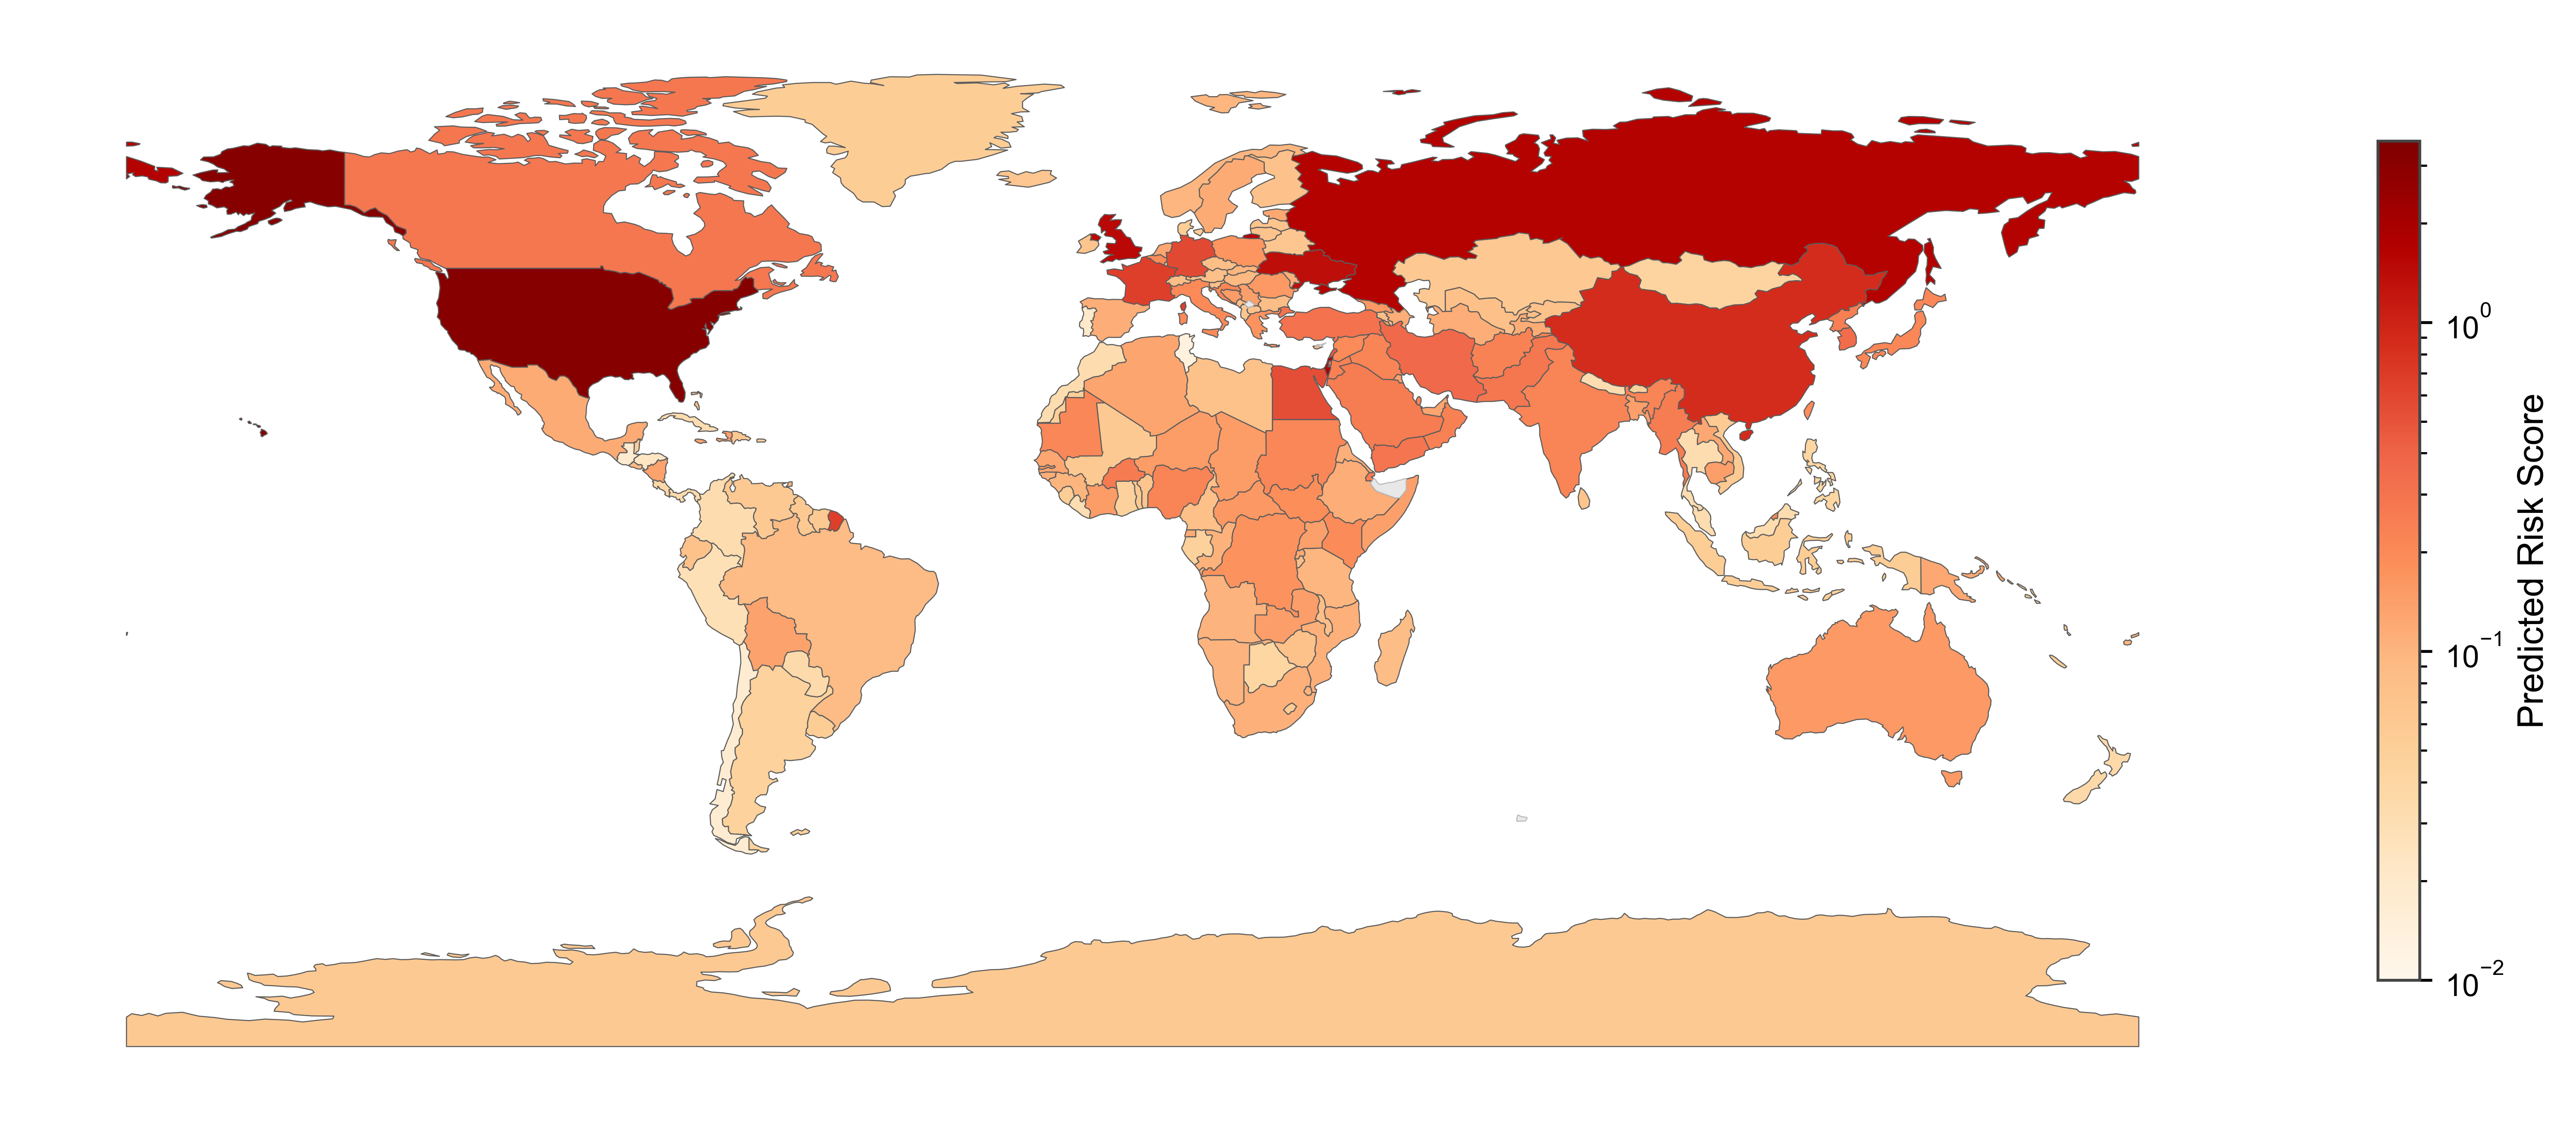
\includegraphics[width=0.92\linewidth]{risk_map_2024.png}%
}{%
  \fbox{\parbox[c][4.5cm][c]{0.92\linewidth}{\centering \textit{figures/risk\_map\_2024.png}\\ predicted 2024 risk for all 247 countries}}%
}
\caption{Predicted 2024 geopolitical risk for all 247 countries, including the 203 with no official index. Color is log scaled so the heavy tailed extremes do not wash out the rest.}
\label{fig:map}
\end{figure}

\begin{table}[H]
\caption{Top 2024 Risk Scores, Labeled and New Countries}
\label{tab:scores}
\centering
\begin{tabular}{lcc}
\toprule
\textbf{Country} & \textbf{Official GPR} & \textbf{Predicted risk} \\
\midrule
United States & 3.15 & 3.11 \\
Israel & 1.92 & 1.95 \\
Russian Federation & 1.62 & 1.66 \\
United Kingdom & 1.52 & 1.50 \\
Ukraine & 1.41 & 1.39 \\
China & 0.87 & 0.87 \\
\midrule
Lebanon & none & 0.47 \\
Iran & none & 0.35 \\
Yemen & none & 0.30 \\
Burkina Faso & none & 0.29 \\
\bottomrule
\end{tabular}
\end{table}

\subsection{Model Selection Results}
XGBoost wins both tests. It ranks unseen countries at 0.81, against 0.74 for the Random Forest and 0.64 for the linear model. On the unseen-year test the three are closer, but XGBoost still leads. All three beat the predict-the-average baseline by a wide margin, which confirms the features have signal. Table \ref{tab:models} has the full comparison.

\begin{table}[H]
\caption{Model Comparison on Two Validation Schemes}
\label{tab:models}
\centering
\begin{tabular}{lcccc}
\toprule
& \multicolumn{2}{c}{\textbf{Unseen countries}} & \multicolumn{2}{c}{\textbf{Unseen years}} \\
\cmidrule(lr){2-3}\cmidrule(lr){4-5}
\textbf{Model} & \textbf{Spearman} & \textbf{MAE} & \textbf{Spearman} & \textbf{MAE} \\
\midrule
XGBoost & 0.81 & 0.16 & 0.91 & 0.11 \\
Random Forest & 0.74 & 0.18 & 0.91 & 0.12 \\
ElasticNet & 0.64 & 0.24 & 0.85 & 0.14 \\
Baseline (predict mean) & n/a & 0.27 & n/a & 0.28 \\
\bottomrule
\end{tabular}
\end{table}

\subsection{Forecasting Accuracy}
The scorer is almost perfect in calm years, with an error around 0.045 from 2019 to 2021, and across all 264 forecasts the correlation is 0.91 with an error of 0.11. One year stands out, 2022, where the error jumps to 0.30. That is the Russia and Ukraine shock, and no model catches it a year ahead, because the features do not move that fast. The scorer's weakness is sudden onset, but the detector covers it. Table \ref{tab:years} has the year-by-year numbers.

\begin{table}[H]
\caption{Expanding-Window Forecast Accuracy by Year}
\label{tab:years}
\centering
\begin{tabular}{lccc}
\toprule
\textbf{Forecast year} & \textbf{Train years} & \textbf{Spearman} & \textbf{MAE} \\
\midrule
2019 & 4 & 0.92 & 0.045 \\
2020 & 5 & 0.95 & 0.041 \\
2021 & 6 & 0.94 & 0.050 \\
2022 & 7 & 0.92 & 0.300 \\
2023 & 8 & 0.87 & 0.130 \\
2024 & 9 & 0.94 & 0.092 \\
\midrule
Pooled & n/a & 0.91 & 0.110 \\
\bottomrule
\end{tabular}
\end{table}

\subsection{Anomaly Detector Validation}
The z-score and the Isolation Forest tie at 43 of 50, and the Local Outlier Factor fails at 17 of 50, which fits the known weakness of density methods in many dimensions. A statistical method matches the machine-learning one, so I keep both, the Isolation Forest as the model and the z-score as the readable check. To rule out luck I ran the permutation test: a chance detector catches about 20 of 50, so 43 of 50 with a p value below 0.001 is real skill, not over-flagging. Table \ref{tab:detect} has the comparison.

On timing, the detector fires about three months before the Russia and Ukraine invasion, since the buildup shows up in the news first. Figure \ref{fig:ukraine} shows Ukraine crossing the alert bar in November 2021. Sudden events like coups have no buildup, so the detector fires the same month. The alert count also rises in turbulent periods and falls in calm ones, which is what it should do. Early warning for slow-building crises and same-month detection for sudden ones.

\begin{figure}[H]
\centering
\IfFileExists{figures/anomaly_ukraine_2022.png}{%
  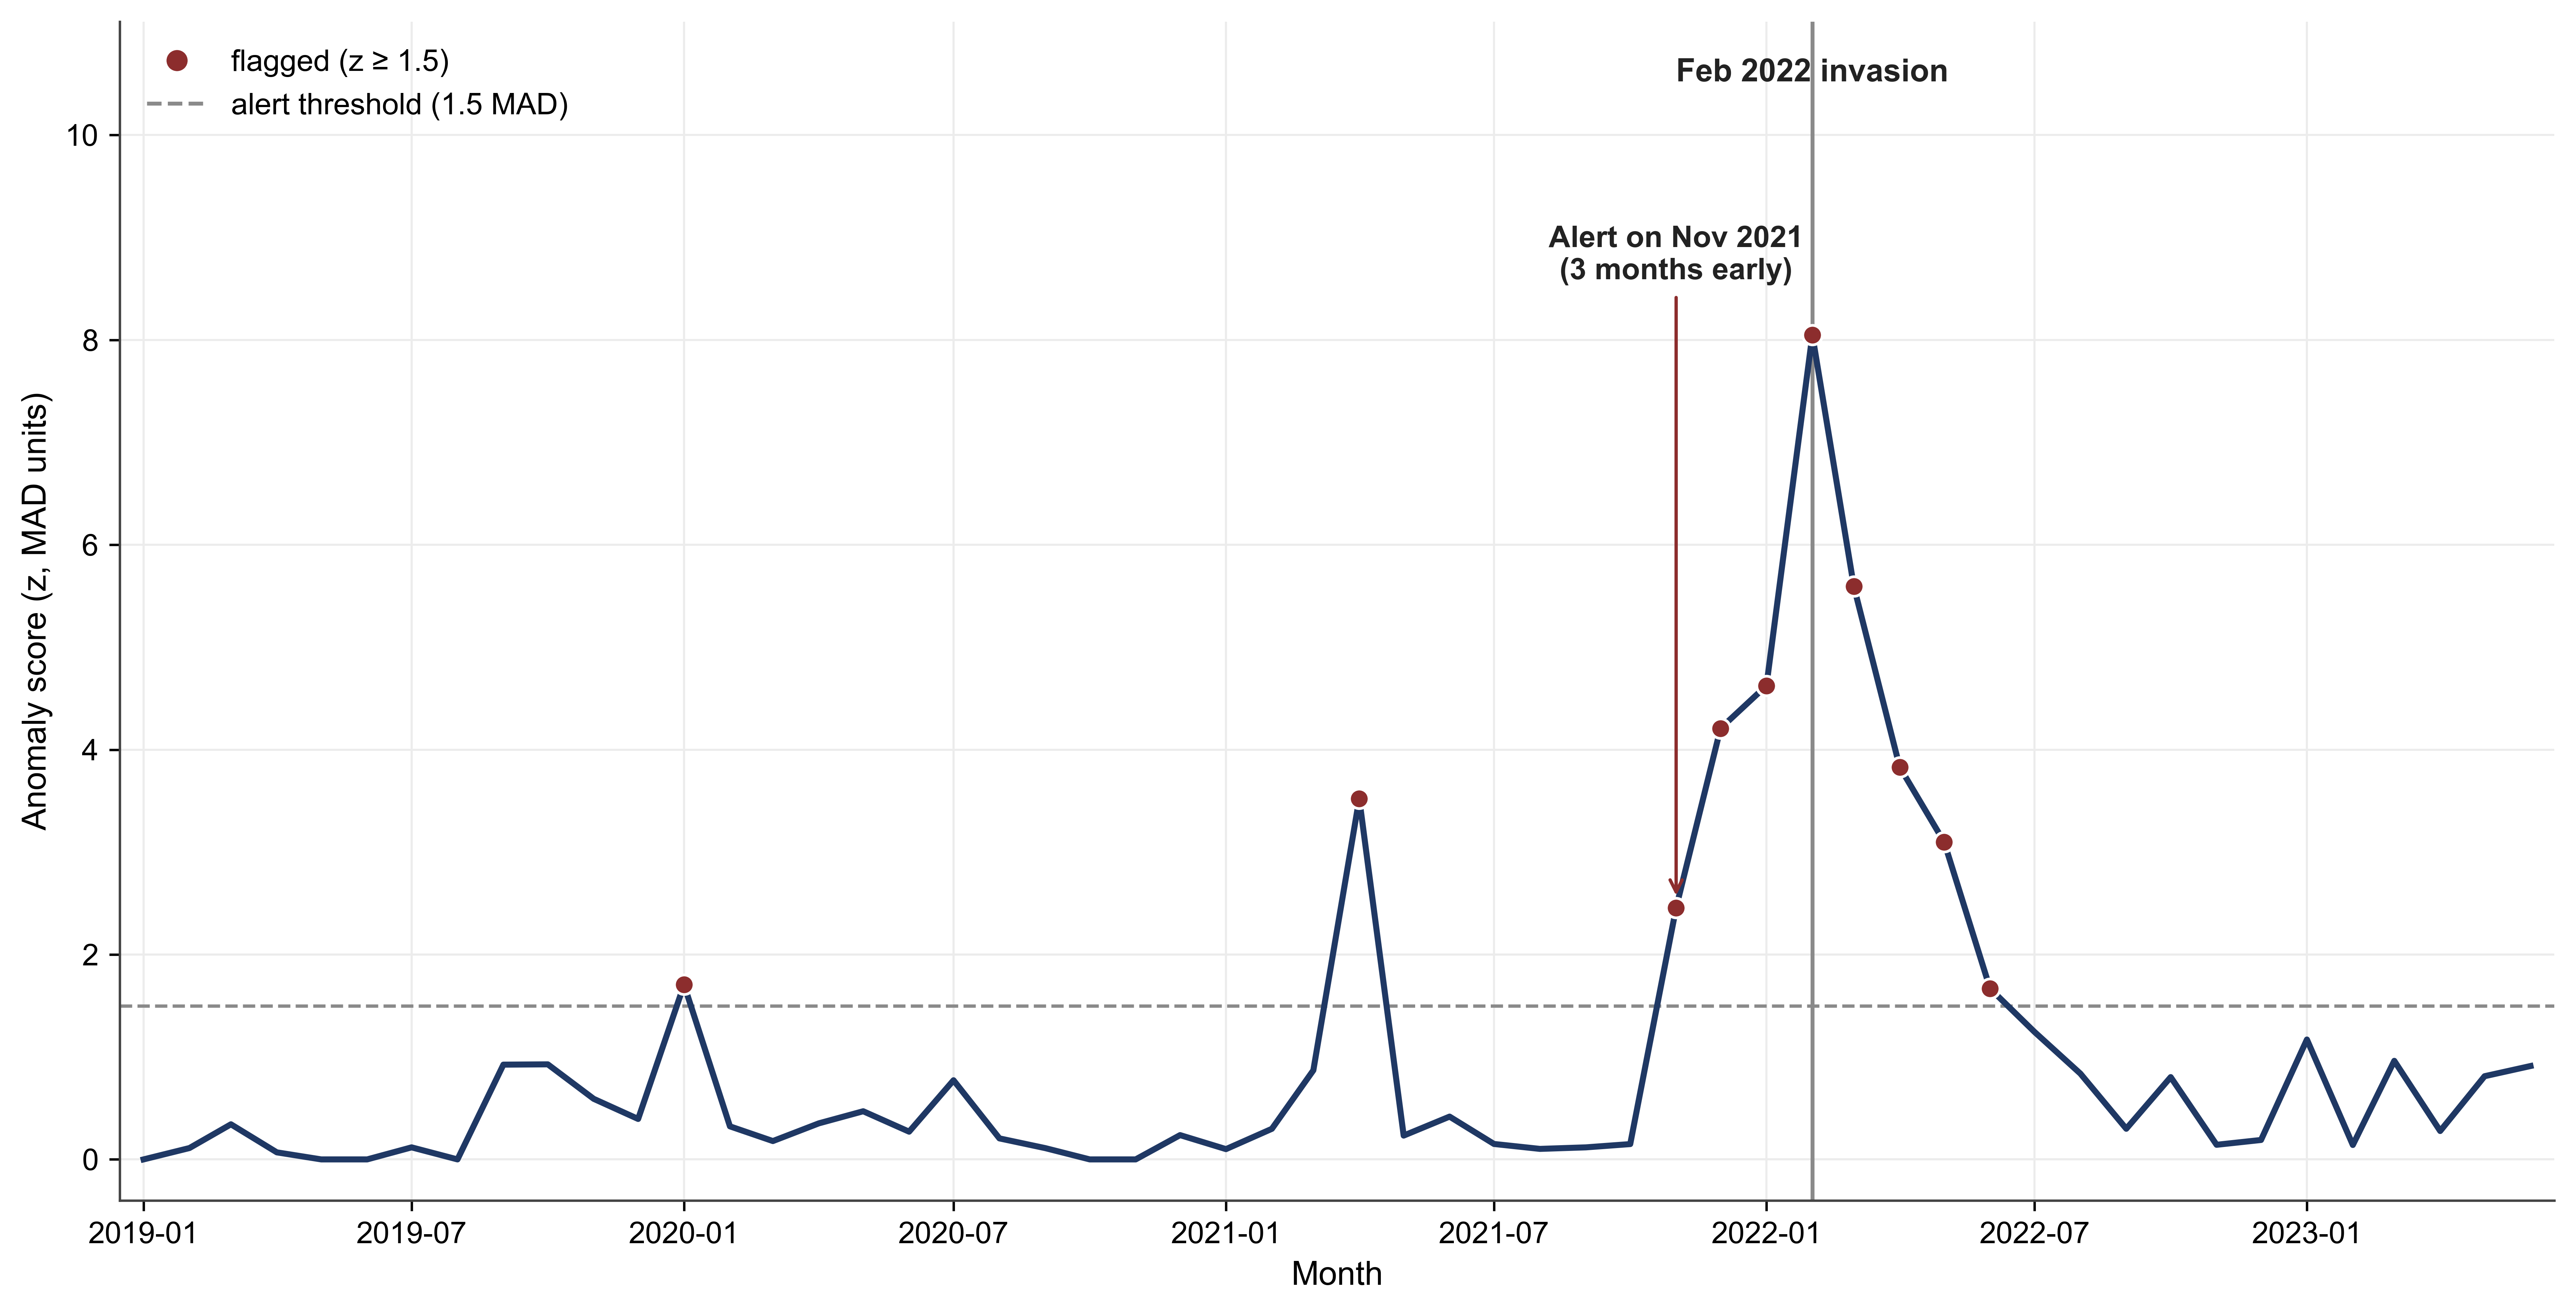
\includegraphics[width=0.95\linewidth]{anomaly_ukraine_2022.png}%
}{%
  \fbox{\parbox[c][4cm][c]{0.95\linewidth}{\centering \textit{figures/anomaly\_ukraine\_2022.png}\\ Ukraine anomaly score around the 2022 invasion}}%
}
\caption{Ukraine's monthly anomaly score around the 2022 invasion. The score crosses the alert bar in November 2021, three months early, and the spring 2021 flag lines up with the earlier Russian troop buildup.}
\label{fig:ukraine}
\end{figure}

\begin{table}[H]
\caption{Detector Comparison on 50 Known Crisis Onsets}
\label{tab:detect}
\centering
\begin{tabular}{lccc}
\toprule
\textbf{Method} & \textbf{Detected} & \textbf{Rate} & \textbf{Beats chance} \\
\midrule
z-score (baseline) & 43 / 50 & 0.86 & yes, $p<0.001$ \\
Isolation Forest (ML) & 43 / 50 & 0.86 & yes, $p<0.001$ \\
Local Outlier Factor (ML) & 17 / 50 & 0.34 & no \\
Chance (permutation) & $\approx$ 20 / 50 & 0.40 & n/a \\
\bottomrule
\end{tabular}
\end{table}

\subsection{Limitations}
The scorer cannot replicate the level of the most extreme countries, only their rank, since a tree cannot predict past the range it trained on, so the top powers sit a little below the line even though their order holds. The scores for the 203 uncovered countries are best read as a ranking among themselves, not as values directly comparable to the 44 labeled powers. GDELT is noisy, with field accuracy near 55 percent \cite{hong2025}, which is why I work with shares and per-country baselines. The GPR target carries an Anglo media view \cite{caldara2022}, so low-coverage countries are harder to place. And the detector test measures recall, it catches the crises, but not precision, which needs a full conflict label set to measure properly.

\section{Ethical Considerations}
This project is built for public good, as an aid for analysts, not for targeting anyone or for real use before it is fully validated. I am open about its limits. Fairness is a real concern, since the GPR target carries a Western media bias that can misplace low-coverage countries. The work uses country-level data only, with no individual data, so it does not risk anyone's privacy. I cite every dataset and respect each provider's terms, including the non-commercial and no-redistribution rules on the Global Sanctions Data Base.

\section{Conclusion}
I built one system with two parts: a scorer that rates country risk from structural features, and a detector that flags emerging unrest from monthly news. The scorer ranks unseen countries at 0.81, forecasts the next year at 0.91, and extends a score to the 203 countries with no published index. Its weak spot is the sudden onset year, 2022, and the detector covers exactly that gap, catching 43 of 50 known crises and giving a few months of warning on slow-building ones. This kind of tool is best used as an aid to analysis, not a predictor of exact events \cite{murphy2024}. For future work, I plan to test the detector's precision against a second conflict dataset like ACLED, and build an interactive dashboard that displays each country's risk score and its latest monthly unrest alerts.

\section{Use of AI Tools}
Anthropic's LLM \enquote{Claude} was used for coding help and polishing notebooks. All analysis, interpretation, and writing decisions are my own, and all text is in my own words.

\bibliographystyle{apacite}
\bibliography{references}

\end{document}
